\section{Materiales Inteligentes}
\subsection{Aspectos historicos}
Los materiales inteligentes, también conocidos como materiales activos, adaptativos o responsivos, han sido objeto de investigación y desarrollo en diversas disciplinas a lo largo de la historia. Según \cite{materiales} estos materiales tienen la capacidad de responder de manera adaptativa a estímulos externos, como cambios de temperatura, presión, luz, electricidad, entre otros. Aquí hay un breve resumen de algunos hitos históricos en el desarrollo de materiales inteligentes:
    \begin{itemize}
        \item En la década de 1960, se desarrollaron y aplicaron ampliamente materiales piezoeléctricos, que tienen la capacidad de generar una carga eléctrica en respuesta a la aplicación de presión mecánica. Estos materiales se utilizan en sensores y actuadores.
        \item Se produjo un avance significativo con el descubrimiento de polímeros electroactivos, como los polímeros conductores y los electrocerámicos. Estos materiales tienen propiedades eléctricas que pueden ser controladas por estímulos externos.
        \item Los materiales con memoria de forma, como las aleaciones de níquel-titanio (conocidas como Nitinol), fueron desarrollados en esta década. Estos materiales tienen la capacidad de recordar y recuperar su forma original después de ser deformados, lo que ha llevado a aplicaciones en la industria biomédica y aeroespacial.
        \item En las últimas décadas, ha habido un aumento en la investigación de biomateriales inteligentes que responden a estímulos biológicos. Estos materiales se utilizan en aplicaciones médicas, como sistemas de liberación controlada de medicamentos.
        \item Se han desarrollado materiales inteligentes que responden a condiciones ambientales, como cambios de temperatura, humedad o luz solar. Estos materiales tienen aplicaciones en la construcción, la arquitectura y la ingeniería civil.
        \item Los materiales inteligentes tienen aplicaciones en una variedad de campos, incluyendo la robótica, la electrónica flexible, la fabricación avanzada, la industria automotriz y la ingeniería estructural.
    \end{itemize}
\subsection{Métodos de obtención}
    \subsubsection{Síntesis Química}
    Muchos materiales inteligentes se obtienen a través de métodos químicos, que pueden incluir la mezcla y reacción de componentes específicos para formar el material deseado. Esto puede incluir la síntesis de polímeros conductores, compuestos termocrómicos, y otros materiales sensibles a estímulos.
    \subsubsection{Procesamiento de Aleaciones}
    Para materiales con memoria de forma como Nitinol (aleación de níquel-titanio), se utilizan procesos metalúrgicos para obtener la aleación deseada. Esto puede incluir la fusión y solidificación controlada de los metales para lograr las propiedades deseadas.
    \subsubsection{Deposición de Películas Delgadas}
    Para aplicaciones en dispositivos electrónicos y ópticos, se utilizan métodos de deposición de películas delgadas, como la deposición física de vapor (PVD) o la deposición química de vapor (CVD), para producir capas delgadas de materiales con propiedades específicas.
    \subsubsection{Fabricación Aditiva (Impresión 3D)}
    La fabricación aditiva, o impresión 3D, se utiliza para crear estructuras complejas de materiales inteligentes. Puede ser especialmente útil para polímeros y ciertos compuestos sensibles a estímulos.
    \subsubsection{Electroquímica}
    Algunos materiales inteligentes, como electrorreológicos y cromóforos electrocrómicos, se obtienen mediante métodos electroquímicos. Esto implica la manipulación de las propiedades del material mediante la aplicación de corriente eléctrica.
    \subsubsection{Síntesis Biológica}
    En algunos casos, se utilizan métodos biológicos para obtener materiales inteligentes. Esto puede incluir la ingeniería genética de microorganismos o el uso de organismos vivos para producir materiales específicos.
\subsection{Transformaciones de estado}
Los materiales inteligentes exhiben diversas transformaciones de estado en respuesta a estímulos específicos. Estas transformaciones son esenciales para su funcionalidad adaptativa.
    \begin{itemize}
        \item Algunos materiales, como las aleaciones de níquel-titanio (Nitinol) y ciertos polímeros, pueden experimentar un cambio reversible en su forma en respuesta a cambios de temperatura. Este fenómeno se conoce como memoria de forma, y permite a estos materiales recuperar su forma original después de ser deformados.
        \item Los materiales inteligentes a menudo exhiben cambios en sus propiedades eléctricas en respuesta a estímulos externos \cite{castagnino-mat-nanotecnologia}. Los polímeros conductores y los materiales piezoeléctricos son ejemplos. Estos materiales pueden cambiar su conductividad eléctrica o generar una carga eléctrica en respuesta a factores como presión, temperatura o campos eléctricos.
        \item Algunos materiales inteligentes, como los fotocrómicos y termocrómicos, pueden cambiar de color en respuesta a la exposición a la luz o al calor. Estos materiales encuentran aplicaciones en la fabricación de lentes de sol, ropa que cambia de color con la temperatura, entre otras.
        \item Los materiales que responden a la humedad, conocidos como hidrorespóndicos, pueden experimentar cambios en su volumen en presencia de agua. Estos materiales son utilizados en aplicaciones como sensores de humedad y actuadores biomiméticos.
        \item Algunos geles y polímeros inteligentes pueden experimentar un cambio en su rigidez o viscosidad en respuesta a estímulos como cambios de pH, temperatura o concentración iónica. Estos materiales son utilizados en la fabricación de actuadores y dispositivos biomédicos.
        \item Los materiales termoeléctricos pueden cambiar su tamaño en respuesta a cambios de temperatura. Este fenómeno se utiliza en algunos sistemas de refrigeración termoeléctrica y en dispositivos microelectromecánicos (MEMS).
        \item Algunos materiales termocrómicos pueden experimentar un cambio de fase en respuesta a cambios de temperatura, lo que resulta en un cambio en sus propiedades ópticas, como el color. Estos materiales son utilizados en aplicaciones como recubrimientos que indican la temperatura.
    \end{itemize}
\subsection{Clasificación de los Materiales Inteligentes}
    \subsubsection{Materiales con memeria de forma}
    Estos materiales pueden cambiar su forma de manera reversible en respuesta a un estímulo específico, como cambios de temperatura. Este cambio de forma es posible debido a una transformación cristalina reversible en el material.
    \subsubsection{Polimeros inteligentes}
    Los polímeros inteligentes pueden cambiar sus propiedades físicas, químicas o eléctricas en respuesta a estímulos externos. Por ejemplo, algunos polímeros conductores pueden alterar su conductividad eléctrica cuando se exponen a campos eléctricos o cambios de temperatura.
    \subsubsection{Materiales piezoelectricos}
    Los materiales piezoeléctricos generan una carga eléctrica cuando se deforman mecánicamente y, a su vez, experimentan una deformación mecánica cuando se les aplica un campo eléctrico.
    \subsubsection{Materiales Termocrómicos y Fotocrómicos}
    Los materiales termocrómicos cambian de color en respuesta a cambios de temperatura, mientras que los fotocrómicos cambian de color cuando se exponen a la luz. Estos materiales encuentran aplicaciones en gafas, textiles y sensores.
    \subsubsection{Materiales Magnetoestrictivos}
    Los materiales magnetoestrictivos experimentan un cambio en sus dimensiones en respuesta a un campo magnético. Este fenómeno se utiliza en actuadores y sensores magnéticos.
    \subsubsection{Materiales Ópticos cambiantes}
    Cambian sus propiedades ópticas, como la transmitancia de luz, en respuesta a cambios de temperatura o campos eléctricos. Se utilizan en pantallas de cristal líquido y dispositivos ópticos.
    \subsubsection{Materiales Hidrorespóndicos}
    Estos materiales pueden cambiar su volumen en respuesta a cambios en la humedad o la presión de agua. Se utilizan en sensores de humedad y aplicaciones biomédicas.
\subsection{Aleaciones de memoria de forma(SMA)}
Las aleaciones con memoria de forma (SMA, por sus siglas en inglés Shape Memory Alloys) son materiales metálicos que tienen la capacidad única de "recordar" y recuperar su forma original después de haber sido deformados. Este comportamiento se debe a una transición de fase martensítica que ocurre reversiblemente en el material. Entre las aleaciones de memoria de forma más comunes se encuentra la aleación de níquel-titanio, conocida comúnmente como Nitinol.
    \subsubsection{Aplicaciones}
        \begin{itemize}
            \item Stents: Utilizados en cirugía cardiovascular, los stents hechos de SMA se pueden comprimir para la inserción y luego recuperar su forma original una vez colocados en una arteria.
            \item Actuadores en Robótica: Las aleaciones de memoria de forma se utilizan en actuadores para lograr movimientos precisos y controlados en aplicaciones robóticas.
            \item Conectores y Enganches: Se utilizan en aplicaciones industriales y aeroespaciales donde se requieren componentes que se puedan acoplar y desacoplar de manera eficiente.
        \end{itemize}
        
        \begin{figure*}[h]
            \centering
            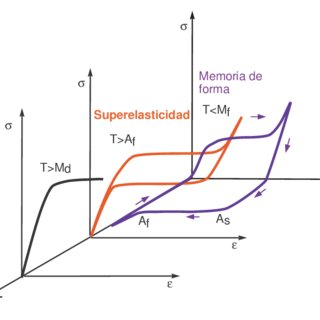
\includegraphics[height=7.8cm]{assets/figures/SMA.jpg}         
        \end{figure*}